\chapter{Implementierung}
Im folgenden Kapitel wird die praktische Implementierung der in der Arbeit erarbeiteten Methode beschrieben. Die Implementierung umfasst dabei die Schnittstelle zum Nutzer, sowie die Erhebung, Verarbeitung und Persistenz von relevanten Daten.
\section{Backend}
Für die Implementierung der Arbeit wurde ein Backend konzipiert, welches Informationen und Bilder von Verkehrskameras für Clients vorenthält. Das Ziel ist es dabei Daten der Straßenverkehrszentrale regelmäßig anzufragen und für den Client zu persistieren. Somit wird ermöglicht, dass der Client auch auf ältere Datensätze der Straßenverkehrszentrale zugreifen kann. Weiterhin ermöglicht soll das Backend die Daten in einem möglichst kompakten Format an den Client senden können, damit auch über schwache zelluläre Netzwerkverbindungen von Clients die Daten relativ zügig empfangen können. 
\subsection{Infrastruktur}
Im Rahmen der Implementierung des Backends wurden diverse Anforderungen an die zu verwendenden Technologien beachtet. So soll die resultierende Anwendung auf dem Apache Server eines geteilten Webhosts laufen. Der Apache Server des Webhosts erlaubt das Ausführen von PHP-Skripten, welche für Anfragen und Verarbeitung von Daten der Straßenverkehrszentrale Baden-Württemberg verwendet werden können. Für die Persistenz von Daten besitzt der Webhost alternativ zum Dateisystem auch eine MySQL-Datenbank.
\begin{figure}[ht]
   \centering
     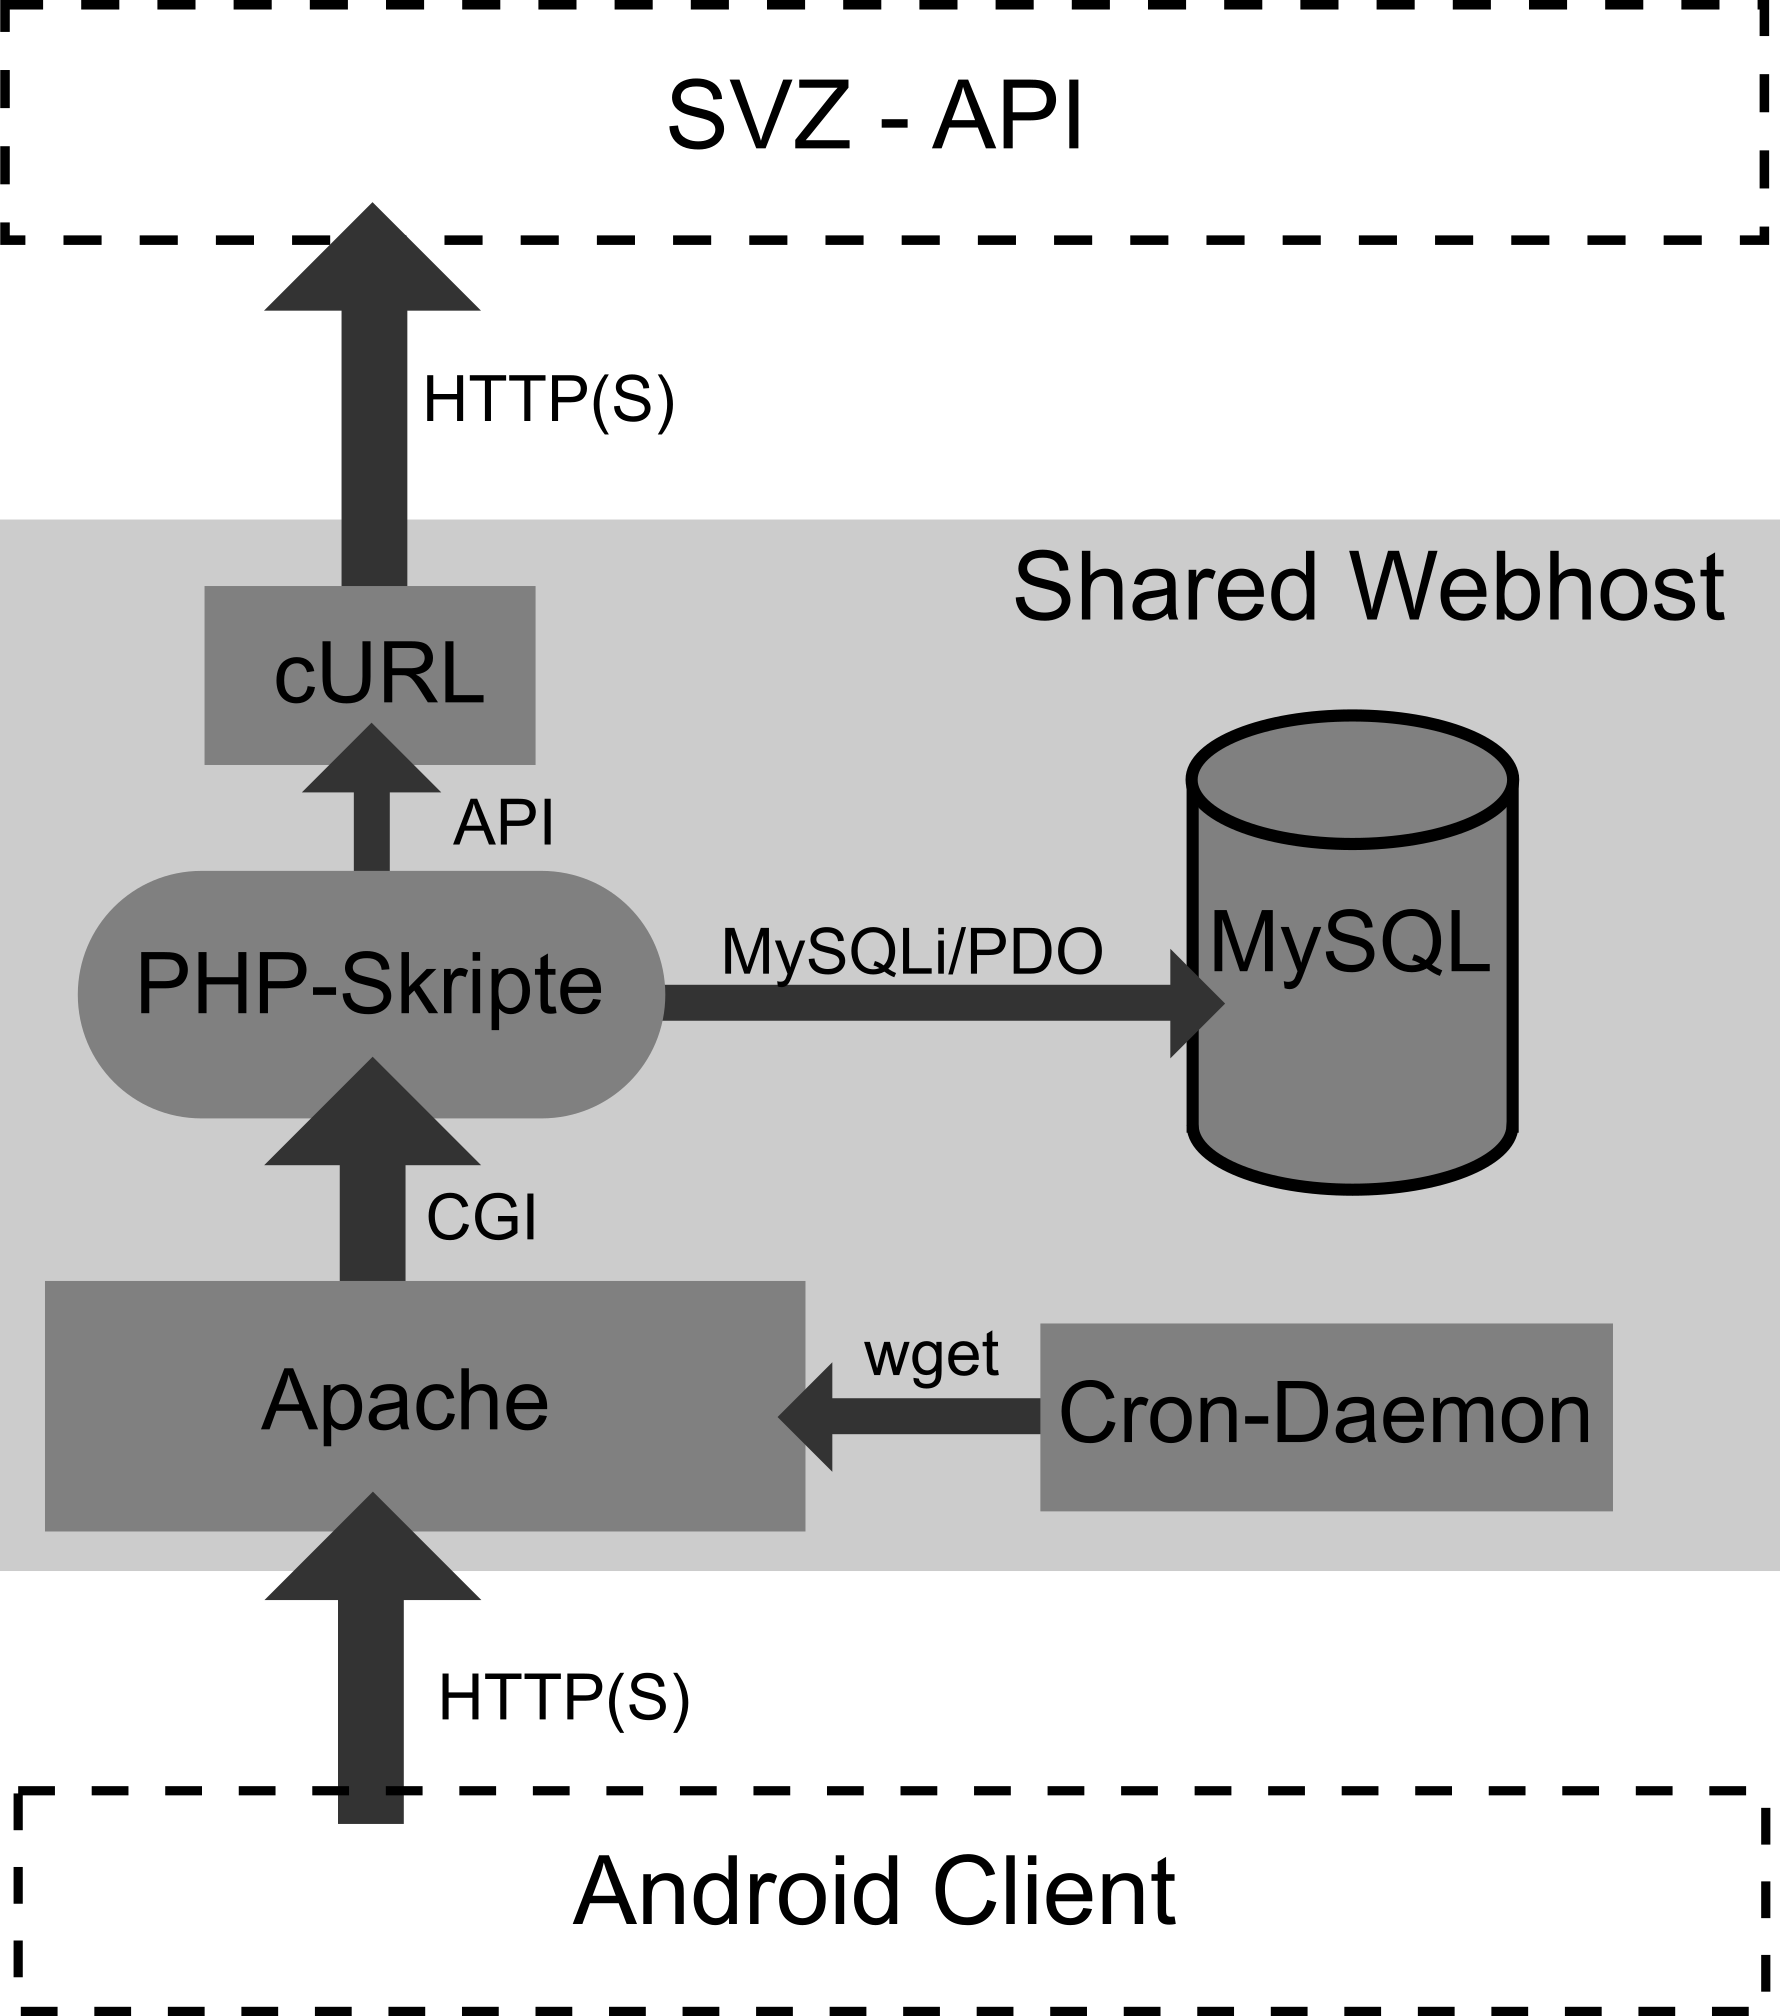
\includegraphics[width=11cm]{Bilder/server-arch} \\
 \caption{Server Architektur}
 \label{fig:serverarch}
\end{figure}

Auf Abbildung~\ref{fig:serverarch} ist zu sehen, dass die Verbindung zum Client über das HTTP-Protokoll verläuft. Der Vorteil ist hierbei, dass das Protokoll bereits von dem Apache Server unterstützt wird und eine Verschlüsselung über TLS eingesetzt werden kann.
\subsection{Datenerhebung}
\label{sec:datenerhebung}
Die Erhebung von benötigten Daten erfolgt durch HTTP-Anfragen an den Server der Straßenverkehrszentrale. Diese können mithilfe der cURL-API in PHP angestoßen werden. Bei "`cURL"' handelt es sich dabei um eine Programm-Bibliothek, mithilfe welcher sich Daten über verschiedene Protokolle übertragen lassen. \newline
Informationen über die jeweiligen Kameras werden über den SVZ-Server in verschieden Formaten bereitgestellt. So sind die Metadaten der Kameras als Textdatei abgespeichert, während die Bilder direkt im JPEG-Format abgerufen werden können. Unter Metadaten der Verkehrskameras sind bei folgende Informationen zu verstehen: 
\begin{itemize}
\item{Eine eindeutige alphanumerische Kamerakennung}
\item{Die entsprechende Autobahnkennung}
\item{Name der nächsten Ausfahrt mit Autobahnkennung}
\item{Position der Kamera}
\end{itemize}
Die Metadaten der Kameras müssen nur einmalig abgerufen und verarbeitet werden, während die Bilder der Verkehrskameras alle 30 Sekunden erneuert werden. Um immer aktuelle Datensätze zu empfangen werden Bilder im 30-Sekunden-Takt angefragt. Dies lässt sich über PHP und einen Cronjob im Linux Betriebssystem des geteilten Webhosts realisieren.
Ein Datensatz der nicht über HTTP-Aufrufe erhoben werden kann sind Masken für Bilder einer Verkehrskameras.
Dabei handelt es sich um Bilder im PNG-Format, welche zur Vorverarbeitung von Bildern verwendet wird. Diese müssen manuell erstellt und in die Datenbank eingepflegt werden, da im Rahmen der Arbeit kein vollständig korrekter Algorithmus zur Automatisierung dieser Aufgabe gefunden wurde.

\subsection{Datenpersistenz}
Für die Persistenz von Daten wurde während der Implementierung auf das Dateisystem verzichtet und nur die MySQL-Datenbank verwendet, da diese die Vorteile einer relationalen Datenbank, sowie sichere Transaktionen bietet.
Bei den Datensätzen die zu persistieren sind handelt es sich dabei um:
\begin{itemize}
\item{Die Metadaten einer Verkehrskamera (siehe \ref{sec:datenerhebung})}
\item{Die Bilder einer Kamera im JPEG-Format}
\item{Die Masken für eine Kamera im PNG-Format}
\end{itemize}
Jeder dieser Datensätze besitzt in der Datenbank eine eigene Tabelle mit einem jeweils eigenen Datenbank-Schema. 
Wichtig bei der Erstellung der jeweiligen Schemata war dabei geeignete Datentypen für die Bilder zu finden, damit diese korrekt und vollständig eingepflegt werden können.
Das Schema für die Datenbank ist auf Abbildung~\ref{fig:dbschema} zu sehen (Primärschlüssel ist fett gedruckt). "`ABID"' bezeichnet dabei die jeweilige Kennung für die Straße. Ein Beispiel hierfür wäre die Autobahnkennung A5.
\begin{figure}[ht]
   \centering
     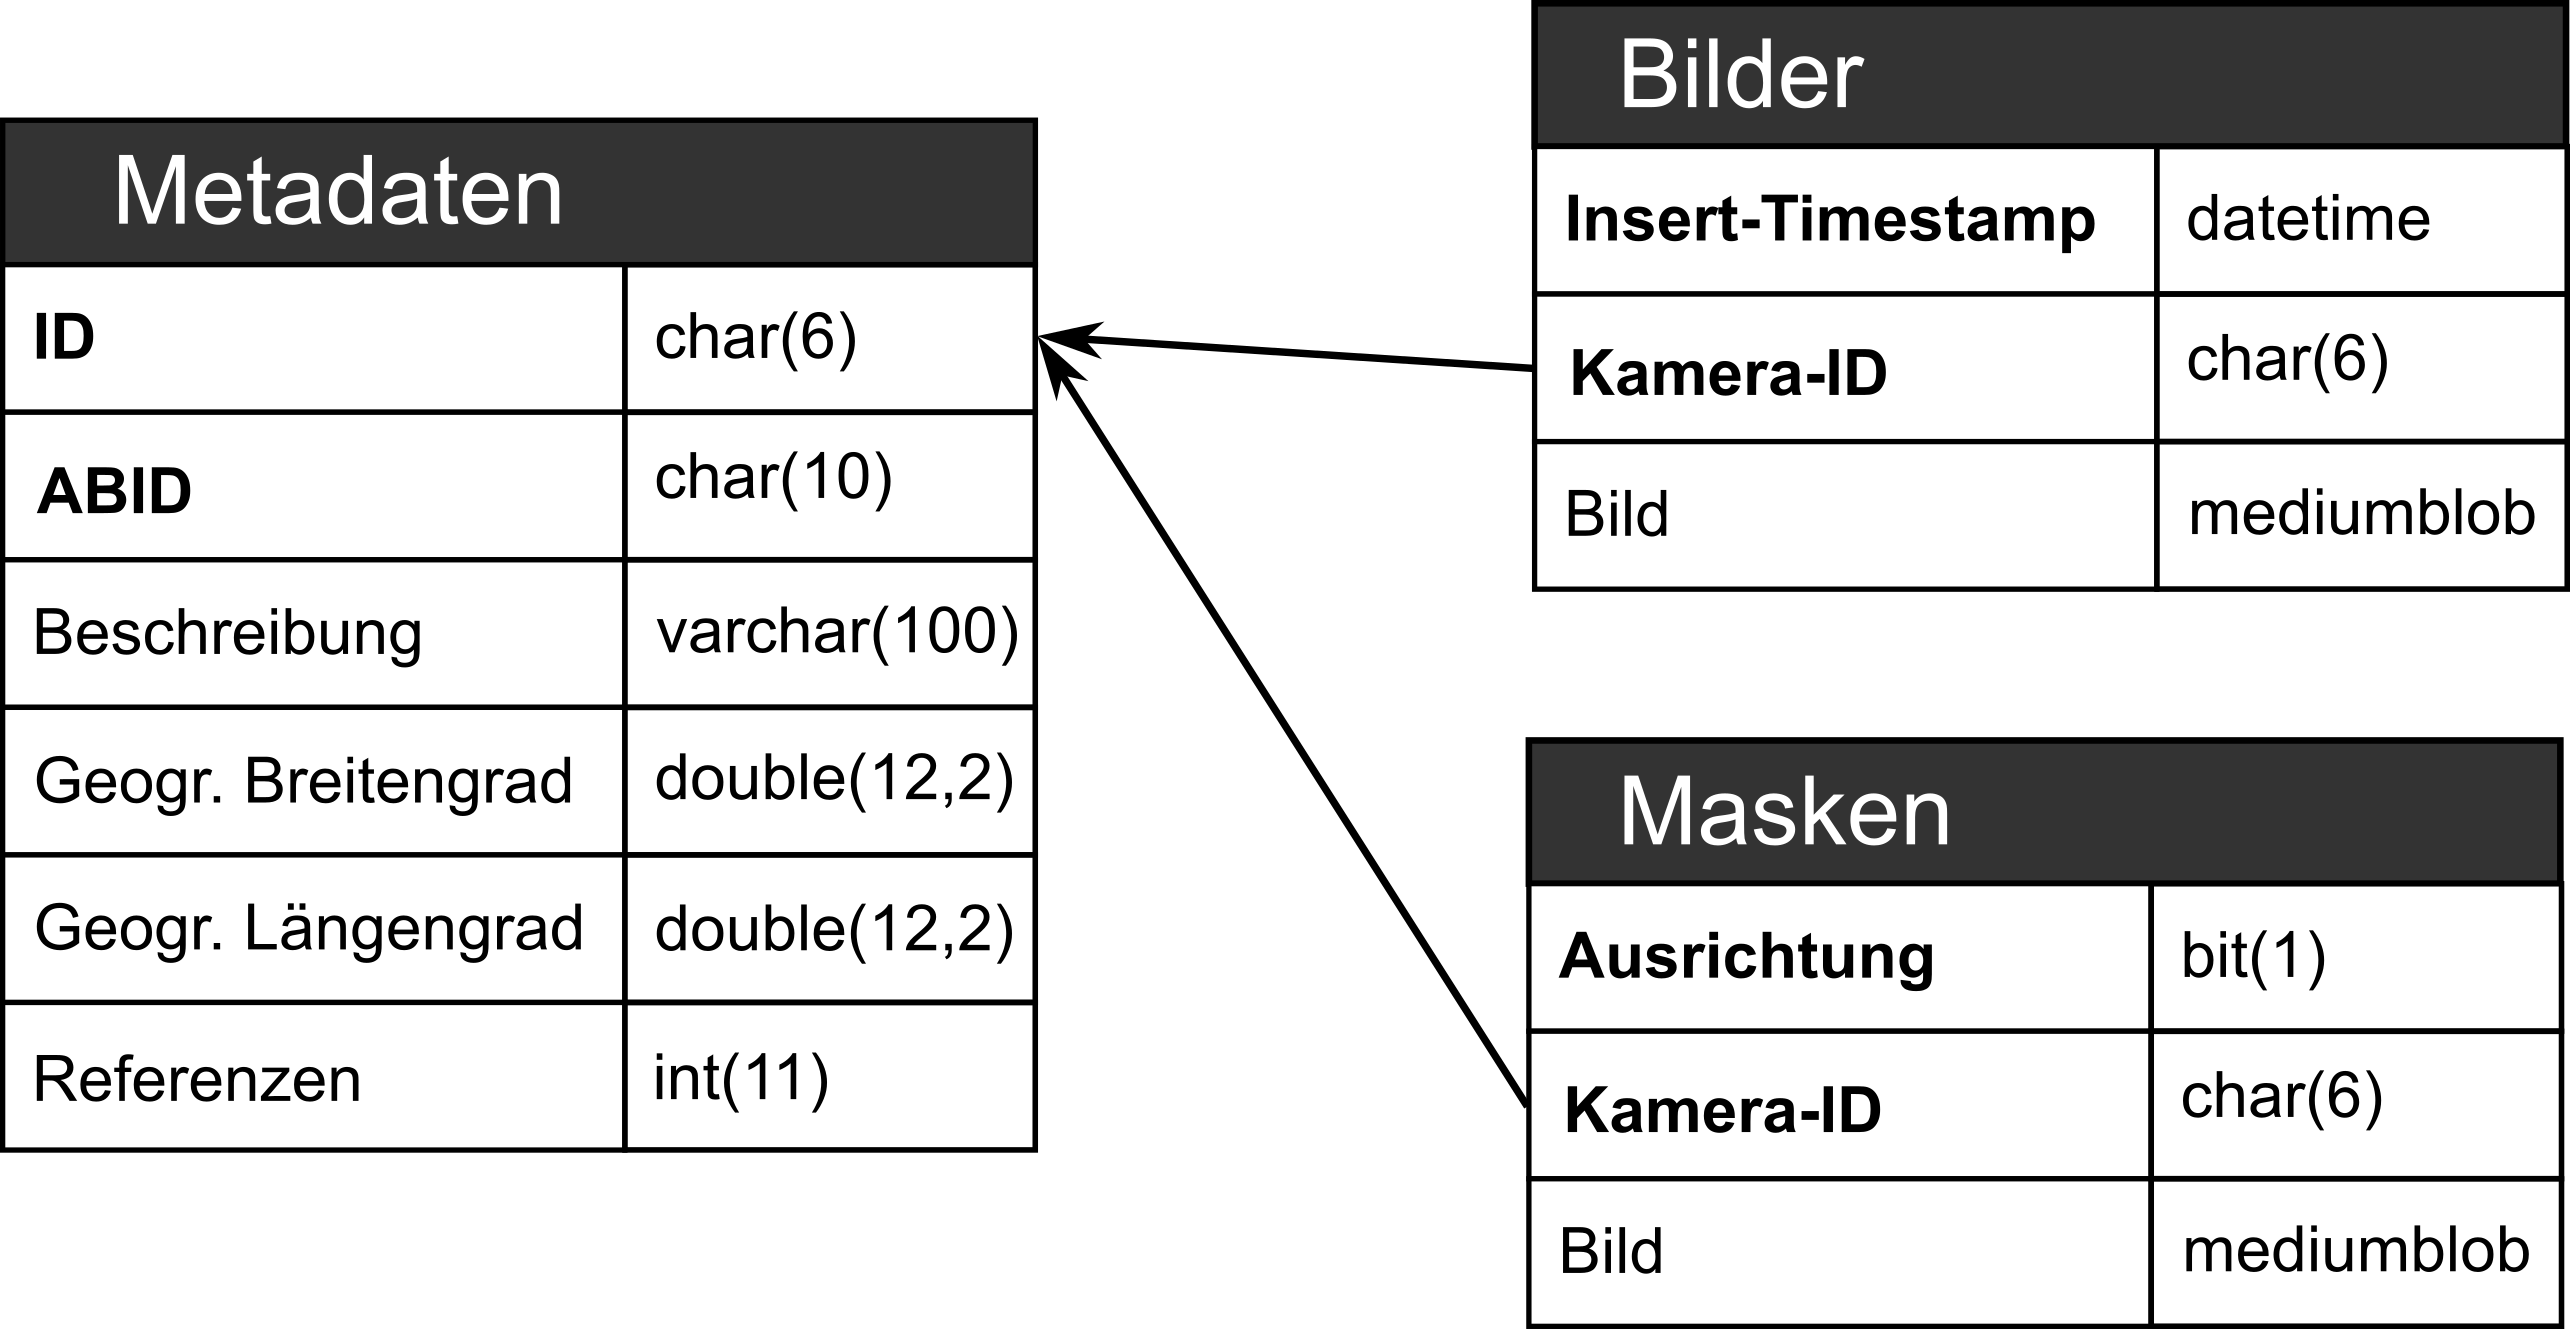
\includegraphics[width=15cm]{Bilder/db-schema} \\
 \caption{Datenbank Schema}
 \label{fig:dbschema}
\end{figure}

\subsection{Datenserialisierung}



\section{Client}
Der Client wird als eine Android Anwendung realisiert, die durch Kommunikation mit dem Backend und der Straßenverkehrszentrale das Problem der Stauerkennung so effizient und ressourcensparend wie möglich löst.
Durch das Verlagern der Berechnungen auf das mobile Endgerät bleibt die Last des Backends gering und die Rechenleistung des Smartphones wird soweit ausgeschöpft, dass Berechnungen effizient, aber sparsam durchgeführt werden können.

\subsection{OpenCV}
Der Kern der Verarbeitung wird durch Algorithmen der OpenCV Bibliothek~\ref{sec:OpenCV} umgesetzt.
Da OpenCV primär als native Bibliothek zur Verfügung steht, bzw. die für Android nutzbare Java-Schnittstelle auf die native (in C++ geschriebene) Implementierung
zurückgreift, muss OpenCV für die jeweiligen Prozessoren der Android Geräte kompiliert werden, auf denen die Anwendung genutzt werden soll.

Eigentlich bietet OpenCV selbst bereits vorkompilierte Versionen der Bibliothek für alle gängigen CPUs und Android Geräte an, jedoch sind diese nicht vollständig.
OpenCV besteht nämlich eigentlich aus zwei teilen: der Kernbibliothek, also OpenCV selbst, aber zusätzlich noch einem Erweiterungsmodul namens {\em OpenCV-Contrib}.

Diese Erweiterung bietet zusätzlich zu den Standartalgorithmen des Kerns Erweiterungen und diverse andere Algorithmen an, welche Randprobleme abdecken und bei der regulären Nutzung der Bibliothek nicht benötigt werden.

Da für die Umsetzung der Anwendung ein spezieller Background-Subtraction Algorithmus benötigt wird, welcher nur in dem Erweiterungsmodul zur Verfügung steht, wird dieses hierfür benötigt.

Die vorkompilierte Version von OpenCV beinhaltet jedoch nicht die Erweiterungen, sodass diese nicht nutzbar ist.

Um die Bibliothek jedoch nicht selbst für jede Architektur kompilieren zu müssen, gibt es die Möglichkeit die Bibliothek von dritten zu beziehen.
Entwickler unter dem Namen {\em QuickBird Studios} stellen auf der Plattform {\em GitHub} (\url{https://github.com/quickbirdstudios/opencv-android} eine aktuelle Version von OpenCV mit allen Erweiterungen zur Verfügung, welche ganz einfach in die App eingebunden und genutzt werden kann.

\subsection{Backend Kommunikation}
\label{sec:BackendCom}
Da das Backend in PHP geschrieben ist, verläuft die Kommunikation über das HTTP-Protokoll an den entsprechenden Webserver.
Android stellt bei der Kommunikation über HTTP jedoch Ansprüche. Die Kommunikation muss auf dem Gerät asynchron geschehen. Das bedeutet, dass im Haupt-Thread,
also dem Programmfaden, welcher für das Darstellen der Oberfläche dient, keinerlei Netzwerkkommunikation geschehen darf, da dies unter Umständen dazu führen könnte, dass die Oberfläche einfriert, da, solange auf das Ende der Kommunikation gewartet wird, die Oberfläche nicht neu dargestellt werden kann.

Um sicherzustellen, dass Kommunikation asynchron verläuft, wird in der Klasse {\em Downloader} jegliche HTTP-Kommunikation gekapselt.
Hierzu wird innerhalb der Klasse ein neuer Thread gestartet, welcher für die Kommunikation zuständig ist. Vor dem Starten des Threads kann ein Callback-Objekt übergeben werden, welches nach Abschluss der Kommunikation die erhaltenen Daten übergeben bekommt und aufgerufen wird.

Ebenfalls stellt der {\em Downloader} sicher, dass pro Instanz der Klasse nur eine Anfrage zur gleichen Zeit abgehandelt werden darf. Dieses Verhalten wird für das spätere Laden der Bilder relevant.
Werden dennoch mehrere Verbindungen gleichzeitig benötigt, können einfach mehrere Instanzen der Klasse erstellt werden.

Um letztendlich mit dem Backend kommunizieren zu können ist der {\em BackendConnector} verantwortlich.
Über den Konstruktor kann die URL des Backends übergeben werden.
Mit Hilfe der {\em Downloader}-Klasse stellt dieser die Endpunkte des Backends als Methoden zur Verfügung:

\begin{itemize}
\item{{\em cameras}: liefert eine Liste aller Unterstützten Kameras zurück}
\item{{\em fetch}: liefert entweder alle gespeicherten Bilder einer Kamera, oder alle Bilder jünger als ein gewünschter Zeitpunkt}
\item{{\em mask}: liefert die Maske für eine Kamera in eine gewünschte Fahrtrichtung}
\end{itemize}

Die Ergebnisse aller Anfragen liegen jedoch im Rohformat als Byte-Array vor. Um die Ergebnisse also nutzen zu können, ist also eine weitere Verarbeitung der Daten in einem späteren Schritt nötig.

\subsection{Geolokalisierung}
Um gezielt Kameras abzufragen und auszuwerten, ist es sinnvoll nur diese auszuwerten, die in unmittelbarer Nähe des Nutzers sind und ebenfalls Relevanz für die Fahrt haben. Hierfür muss demnach die Position des Nutzers ermittelt und ausgewertet werden.

Heutige Smartphones besitzen in der Regel ein GPS-Modul, mit welchem sich die Position bestimmen lässt.
Bevor man jedoch die Möglichkeit hat, mit dem Modul kommunizieren zu können, muss eine Anwendung die erforderlichen Berechtigungen einfordern.
Dafür muss zunächst in der Manifestdatei der Android-Anwendung die Berechtigung {\em android.permission.ACCESS\_FINE\_LOCATION} hinzugefügt werden.
Bei neueren Android-Versionen reicht dies allein jedoch nicht mehr aus. Zusätzlich dazu muss der Nutzer explizit bestätigen, dass die Anwendung Zugriff auf den Standort erhält.

Durch Übergabe des Wertes {\em Manifest.permission.ACCESS\_FINE\_LOCATION} an die Funktion {\em requestPermission} der {\em Activity}-Klasse, die den Einstiegspunkt der Android-Anwendung bietet, wird dem Nutzer ein Dialog angezeigt, durch welchen er Zugriff erteilen oder verweigern kann.


Sind alle Berechtigungen erteilt, so kann die App den Standort abfragen.
Hierfür ist in der App die Klasse {\em GlobalPositionManager} verantwortlich. Diese Kapselt die Interaktion mit dem GPS-Modul und kann über an einen übergeben Callback Standortänderungen regelmäßig nach außen hin kommunizieren.
Hierzu wird zunächst beim {\em LocationManager}, dem System Dienst für die Standortverwaltung des Gerätes, die Lokalisierung angefragt, was dafür sorgt, dass alle 10 Sekunden der aktuelle Standort and den {\em GlobalPositionManager} übergeben wird. Dieser kann anschließend an den Callback übergeben werden und für die weitere Verarbeitung genutzt werden.

\subsection{Richtungsfestellung}
Hat man nun die Position zur Hand, so ist als nächstes relevant zu wissen, wohin gefahren wird, um die zu analysierende Straßenseite zu erkennen.
Hierfür gibt es diverse Ansätze, um das Problem zu lösen.

Beispielsweise stellt Google einen Dienst zur Verfügung, über den bei Übergabe von verschiedenen Positionen die befahrene Straße und Richtung erkannt werden kann. Dieser ist jedoch kostenpflichtig und deshalb nicht geeignet.

Um auch hier den Fokus auf Ressourcensparsamkeit nicht zu verlieren, wurde ein sehr einfacher, jedoch nicht generischer Ansatz gewählt.
Da die Anwendung primär für eine Nutzung auf der A5 gedacht ist, ist das Ziel zunächst nur die Fahrtrichtung auf der A5 zu erkennen.
Auf anderen Autobahnen kann daher nicht ohne Weiteres erkannt werden, auf welcher Straßenseite gefahren wird.

Die A5 erstreckt sich von Niederaula, nördlich von Frankfurt am Main bis nach Weil am Rhein, kurz vor vor der Schweizer Grenze. Grob gesehen kann man sagen sie erstreckt sich von Frankfurt nach Basel.

Um nun die Fahrtrichtung zu erkennen, können die Standorte über die Zeit protokolliert und kumuliert werden, um daraus einen Richtungsvektor zu bilden.
Dieser kann genutzt werden, um abzuschätzen, ob der sich Nutzer Frankfurt oder Basel nähert.

Dazu werden die vom {\em GlobalPositionManager} erfassten Positionen durch die Klasse {\em PositionHistory} protokolliert.
Über die bereitgestellten Methoden {\em getStart} und {\em getEnd} werden die Positionen so aufsummiert, dass Startpunkt und Endpunkt ausgelesen werden können.

Anschließend ermittelt die Klasse {\em DirectionCalculator} die euklidische Norm zwischen sowohl Frankfurt, als auch Basel und den Start- und Endpunkten.
Diese Vernachlässigt zwar die Krümmung der Erdoberfläche und jegliche Höhenunterschiede, ist aber für solch kurze Distanzen völlig ausreichend.

Ist der Startpunkt nun weiter entfernt von Frankfurt als der Endpunkt, so bewegt sich der Nutzer nach Frankfurt, ansonsten in Richtung Basel.

Anfangs ist das Feststellen der Richtung noch recht ungenau. Je mehr Positionen jedoch über die Zeit protokolliert werden, desto genauer wird die Ermittlung der Fahrtrichtung.

Obwohl diese Form der Richtungsfeststellung nur auf der A5 funktioniert, ist die Berechnung sehr effizient und akkurat, da nur wenige einfache Rechenschritte benötigt werden, um somit der Ressourcensparsamkeit gerecht zu werden.

\subsection{Verkehrskameras laden}
Bevor die Informationen zu den Verkehrskameras von der Straßenverkehrszentrale geladen werden können, muss zunächst geprüft werden, welche Kameras das Backend unterstützt.

Hierfür kann über die Klasse {\em AvailableCamerasLoader}, wie im Abschnitt~\ref{sec:BackendCom} beschrieben, über den {\em BackendConnector} mit der Methode {\em cameras} die Liste der unterstützten Kameras abgerufen werden.
Die IDs der Kameras Zeilenweise zurückgeliefert. Der {\em AvailableCamerasLoader} verarbeitet die Zeilen anschließend, sodass eine Liste der verfügbaren Kamera IDs zur verfügung steht.

Zusätzlich dazu werden noch die detaillierten Kamerainformationen der Straßenverkehrszentrale benötigt. Dafür kann über den {\em CameraLoader}, wie im Abschnitt~\ref{sec:AnaCam}, die Liste der Kameras mit dem {\em Downloader} empfangen werden und und verarbeitet werden. Hierfür wird das Tabellenformat aufgeschlüsselt und die benötigten Werte wie ID, Name, Beschreibung und Standort der Kamera in einem {\em Camera}-Modell abgelegt werden.

Da der Standort jedoch ein unterschiedliches Koordinatensystem verwendet, muss dieser jedoch noch konvertiert werden. Hierfür kann über die Bibliothek Proj4J~\cite{proj4j} eine Konvertierung durchgeführt werden.

Diese empfangene Liste wird nun anhand den vom Backend unterstützten Kameras gefiltert, sodass nur noch diese verfügbar sind, mit denen auch gearbeitet werden kann.

Schließlich wird beim aktualisieren der Position des Nutzers, bzw. auch der Fahrtrichtung geprüft, welche Kameras für die weiterfahrt relevant sind. Das bedeutet Kameras die nicht auf der Strecke liegen, werden erst gar nicht benötigt. Liegen Kameras zwar auf der Strecke, aber hinter dem Nutzer, also ist der Nutzer bereits an ihnen vorbei gefahren, so sind diese ebenfalls nicht mehr relevant. Lediglich die Kameras, die vor dem Nutzer auf der Strecke sind, werden für die Stauanalyse benötigt. 
Es wird also nach jeder Positionsänderung geprüft, welche Kameras relevant sind. Diese werden dann Markiert, sodass die spätere Bildanalyse weiß, welche Kameras analysiert werden sollen.

\subsection{Bilder laden}
Das Laden der Bilder gliedert sich in 3 Hierarchiestufen.
Auf der untersten Ebene kann über die {\em fetch}-Methode des {\em BackendConnectors} ein Binärstream an Bilddaten vom Backend für eine Kamera geladen werden.
Da das Backend innerhalb dieses Streams alle Bilder liefert, die es zwischen gepuffert hat, müssen diese zunächst voneinander getrennt werden.

Eine Hierarchieebene darüber regelt der {\em MultiImageLoader} die Verarbeitung.
Nach Erhalt der Rohdaten des Backends wird der Binärstrom aufgespalten.
Jedes Teilbild innerhalb des Stroms hat einen Kopf welcher aus 4 Bytes für die Länge des Bildes und 8 Bytes für den Aufnahmezeitpunkt des Bildes besteht.
Nach den Kopfdaten folgt das eigentliche Bild. Der gesamte Strom besteht nun einer Folge von Kopf und Bild. Wobei zu beachten gilt, dass die Bytereihenfolge des Kopfes {\em Little-Endian} ist, und nicht {\em Big-Endian} wie auf den meisten Android Geräten verwendet.

Es wird also die Länge des Bildes gelesen und konvertiert, danach der Zeitpunkt gelesen und konvertiert und anschließend das Bild über die vorher eingelesene Länge extrahiert. Dieser Vorgang wiederholt sich solange, bis Idealerweise keine Bytes mehr im Strom sind, oder im Fehlerfall die aus dem Kopf entnommene Länge des Bildes länger ist als übrige Bytes im Strom vorhanden sind.

Das Backend liefert standardmäßig jedoch alle Bilder für eine Kamera die es zwischengespeichert hat. Um also nicht bei jeder Anfrage alle Bilder alten Bilder erneut empfangen und verarbeiten zu müssen, wird in der obersten Hierarchiestufe vom {\em CameraImageFetcher} das Strukturierte laden der Bilder koordiniert.

Für jede der relevanten Kameras existiert eine Instanz, die von außerhalb alle 29 aufgefordert wird neue Bilder abzurufen. Das sorgt, dafür, dass mindestens 2 mal innerhalb der Aktualisierungsperiode des Straßenverkehrszentrums auf neue Bilder geprüft wird, um möglichst schnell auf Stau reagieren zu können und die Latenz des Ladens und Verarbeitens der Bilder zu kompensieren.

Die vom {\em MultiImageLoader} empfangenen Bilder werden also zwischengespeichert. Bei einem neuen Abfrageintervall kann über das Durchreichen des Zeitstempels des letzten empfangenen Bildes an den {\em BackendConnector} das Backend dazu instruiert werden, lediglich die Bilder zu senden, die jünger als der besagte Zeitstempel sind.

\subsection{Bilder verarbeiten}
\subsection{Benutzeroberfläche}
\subsection{Text-To-Speech}
\subsection{Bluetooth}
* SCO Headset ausgabe
* Autoverbindung mit Auto
* Service 